\documentclass[conference]{IEEEtran}
\IEEEoverridecommandlockouts

\usepackage{cite}
\usepackage{amsmath,amssymb,amsfonts}
\usepackage{graphicx}
\usepackage{textcomp}
\usepackage{xcolor}
\usepackage{float}
\usepackage{hyperref}
\usepackage{listings}

\def\BibTeX{{\rm B\kern-.05em{\sc i\kern-.025em b}\kern-.08em
    T\kern-.1667em\lower.7ex\hbox{E}\kern-.125emX}}
\begin{document} 


\title{Design of a Simple CS Amplifier}

\author{\IEEEauthorblockN{Emmanuel Jesus R. Estallo}
\IEEEauthorblockA{\textit{Electrical and Electronics Engineering Institute} \\
\textit{University of the Philippines - Diliman}\\
Quezon City, Philippines\\
emmanuel.estallo@eee.upd.edu.ph}}

\maketitle

\section{CS Amplifier} 
\noindent The desired specs are as follows:
\begin{itemize}
	\item $|A_v|>40$ at $V_{DS}=V_{DD}/2=0.9V$
	\item Output swing: $400mV$
	\item Unity-gain frequency: $f_u=100MHz$, $C_L=5pF$
	\item $V^{*}=200mV$
\end{itemize}
\subsection{Selecting $I_D$}
The transconductance can be obtained from:
\begin{equation*}
	g_m = 2\pi f_u C_L
\end{equation*}
this gives us
\begin{equation*}
	g_m = 3.14\; mS
\end{equation*}
The current can be obtained from: 
\begin{equation*}
	V^* = 2\cdot\left( \frac{g_m}{I_D}\right)^{-1} 
\end{equation*} 
and a $V^*$ of $200\; mV$ corresponds to a $g_m/I_D$ of 10. 

\vspace{8pt}
\noindent Thus, 
\begin{equation*}
	I_D = 314\; \mu A
\end{equation*}
\subsection{Choosing the length}
To find the appropriate length, I did a DC sweep on VGS and checked if the intrinsic gain at 
$V^*$ is $> 40$.  
\begin{figure}[H]
	\centering 
	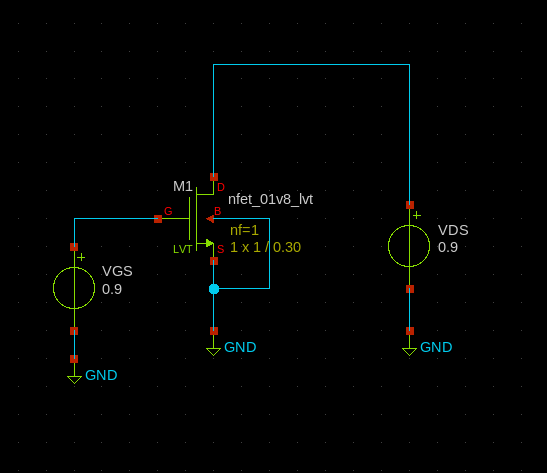
\includegraphics[width=\columnwidth]{schem.png}
	\caption{Schematic diagram}
	\label{schematic}
\end{figure}
At the minimum length, the intrinsic gain is lower than what is desired. We select $L=0.30\mu m$ since it satisfies the specifications. $L=0.25\mu m$ also meets the specifications. However, for a greater swing, the larger length is selected. 
\begin{figure}[H]
	\centering 
	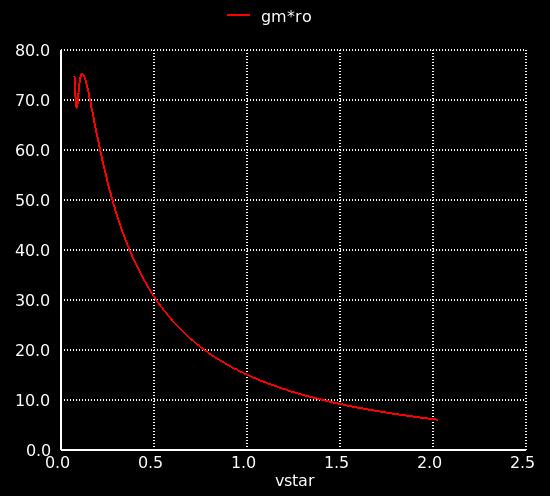
\includegraphics[scale=0.40]{gmro.png}
	\caption{Intrinsic gain}
	\label{gmro}
\end{figure}
The $V^*$ vs $I_D$ plot for a transistor with $W=1\mu m$, $L=0.30 \mu m$ is shown below. 
\begin{figure}[H]
	\centering 
	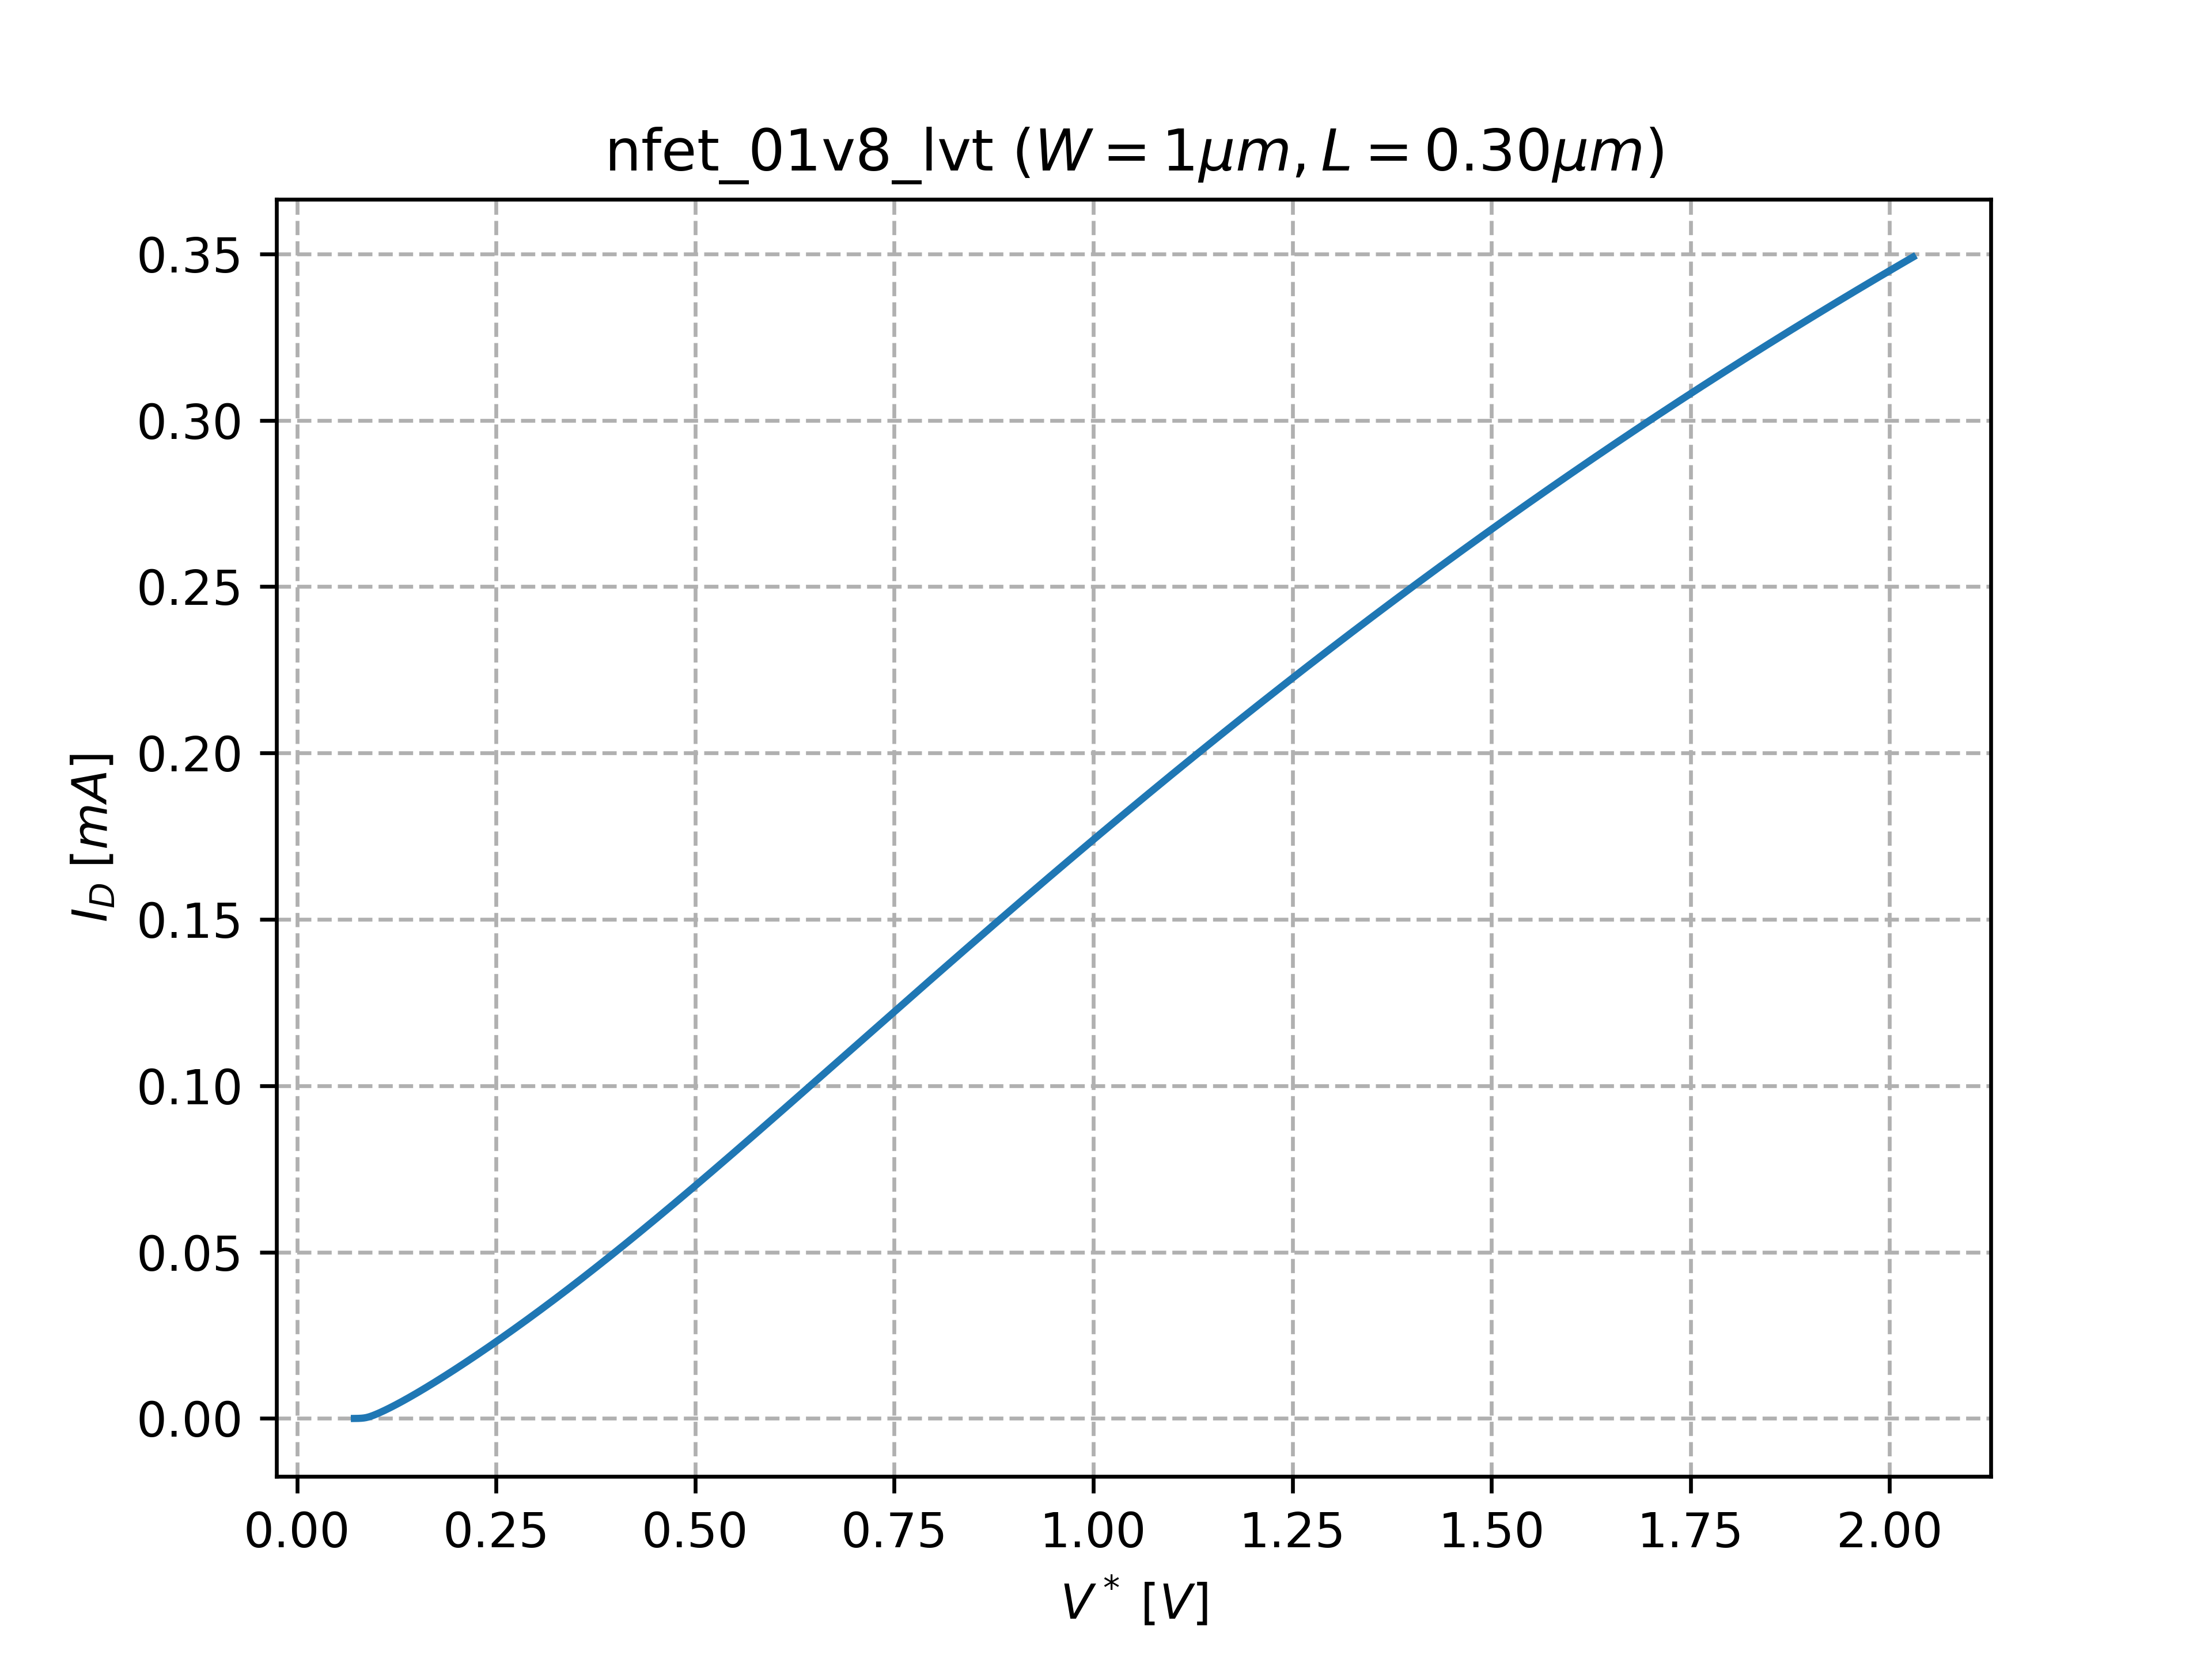
\includegraphics[scale=0.38]{vstar-id.png}
	\caption{$I_D$ vs $V^*$, $W=1\mu m$}
	\label{vstar-id}
\end{figure}
\subsection{Scaling the width}
A python script is used to calculate the scale factor $k_W$ that meets the required $I_D$. The width is scaled using $k_W$. Multiplying the width by $k_W$ scales $I_D$ by approximately the same factor. For this activity, $k_W=21$.
To check, a MEAS directive is used. The required current is $I_D=314\mu A$, what we got is $I_D=345\mu A$, which is quite close. 
\begin{figure}[H]
	\centering 
	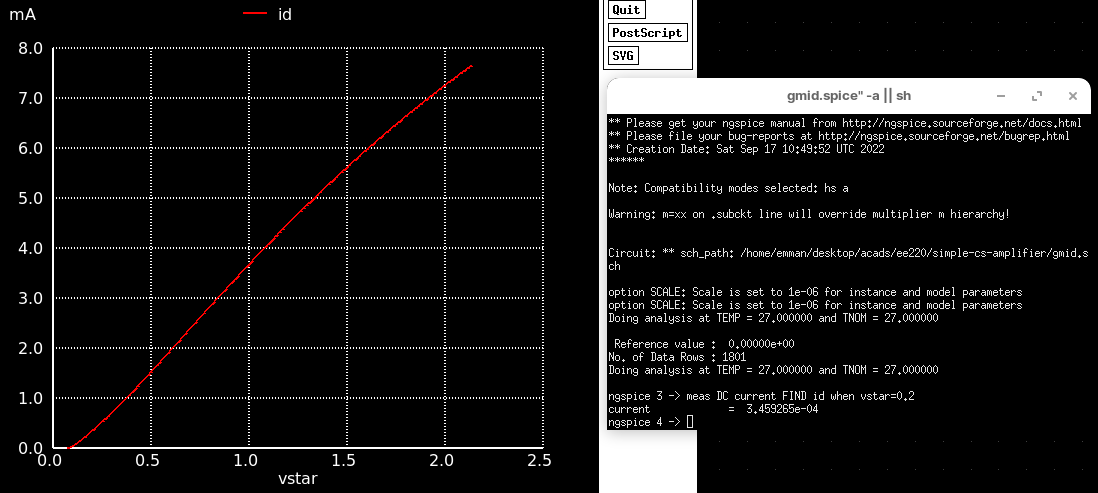
\includegraphics[width=\columnwidth]{vstar-scale-id.png}
	\caption{$I_D$ vs $V^*$, $W=21\mu m$}
	\label{vstar-scale-id}
\end{figure}
\subsection{Output and input swing}
\begin{figure}[H]
	\centering 
	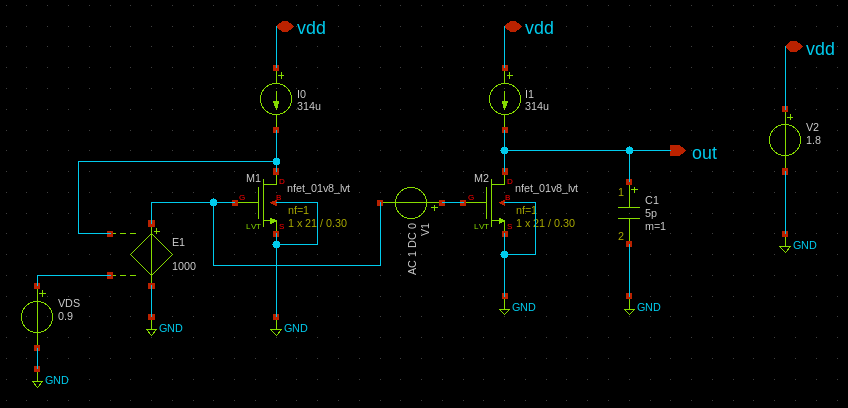
\includegraphics[width=\columnwidth]{schem_large.png}
	\caption{Schematic}
	\label{schem-large}
\end{figure}
To get the input and output swing, we use the schematic in Fig. \ref{schem-large}. Since 
$V_{GS}$ is a function of $V_{DS}$, we can plot $a_o$ vs $V_{DS}$ to get the maximum output
swing and $a_o$ vs $V_{GS}$ to get the corresponding input swing. 

\vspace{8pt}
\subsubsection{Output Swing}
at $V_{DS}\approx 0.52$, $a_o \geq 40$. 
\begin{figure}[H]
	\centering 
	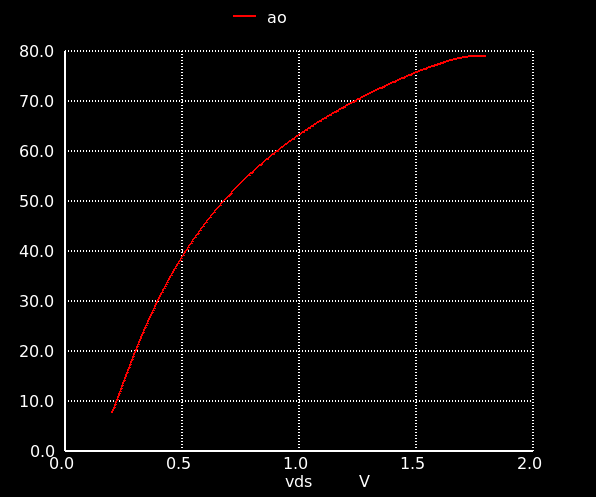
\includegraphics[scale=0.3]{ao-vds.png}
	\caption{$a_o$ vs $V_{DS}$}
	\label{swing-out}
\end{figure}
\subsubsection{Input Swing}
at $V_{GS}\approx 0.71$, $a_o \geq 40$. 
\begin{figure}[H]
	\centering 
	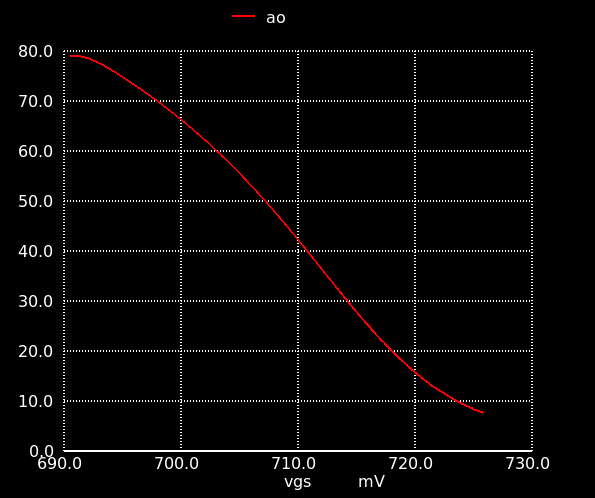
\includegraphics[scale=0.3]{ao-vgs.png}
	\caption{$a_o$ vs $V_{GS}$}
	\label{swing-in}
\end{figure}
Thus, the maximum symmetric output voltage is $0.52 \leq V_{DS} \leq 1.48$ for a total swing of $0.96V$. The corresponding input is $0.69 \leq V_{GS} \leq 0.71$ with a $20mV$ swing.

\subsection{AC analysis}
Using Fig. \ref{schem-large}, an AC sweep from $1 Hz$ to $1GHz$ is used to obtain Fig. \ref{vdb}. Using a MEAS directive, $f_u=104MHz$ which is close to our desired $f_u$. At low frequencies, the gain is $\approx 35dB$
which is $\approx 60\; V/V$
\begin{figure}[H]
	\centering 
	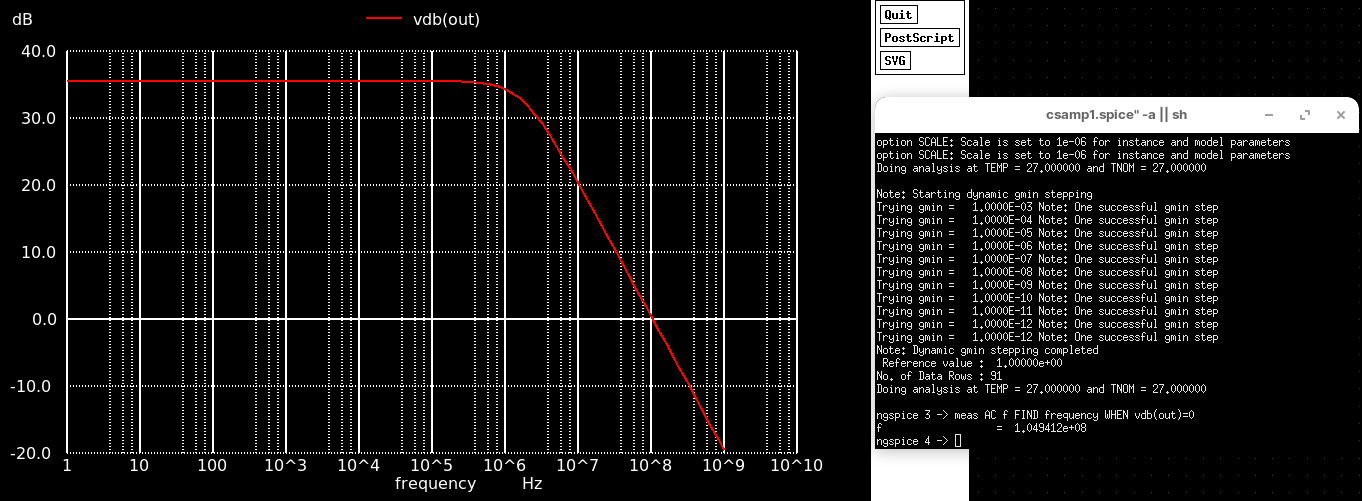
\includegraphics[width=\columnwidth]{vdb.png}
	\caption{Magnitude response}
	\label{vdb}
\end{figure}
\subsection{Discussions}
These are my expected results. Since some values are estimated, there are slight deviations with the desired specifications. 

\vspace{8pt}
\section{CS Amplifier with High $f_t$} 
To get a high $f_t$, we need a high $I_D$ and small $L$. Decreasing $L$ increases $f_t$ if $I_D$
is kept constant. However, since there are no constraints on area and how high $I_D$ could be, the limit would be related to the maximum $W$ that can be used on the PDK. 

\subsection{Selecting the width}
For this PDK, the highest width that can be used is $W=99.9\mu m$. We use this value to get 
the maximum $I_D$. 

\newpage 
\subsection{Choosing the length and $V^*$}
Ideally to get the highest $f_t$, we should select the minimum length. However, the minimum length does not have sufficient intrinsic gain. We use Fig. \ref{schematic} to determine the appropriate length and $V^*$. Since the load is an ideal current source, the gain is only limited by the lower bound $\approx 700mV$. We use $V_{DS}=0.7V$ for the simulation. 

\vspace{8pt}
\subsubsection{$a_o$ vs $V^*$} 
For $0.20\mu m \leq L \leq 0.25\mu m$, the $a_o$ vs $V^*$ plot is shown below. 
\begin{figure}[H]
	\centering 
	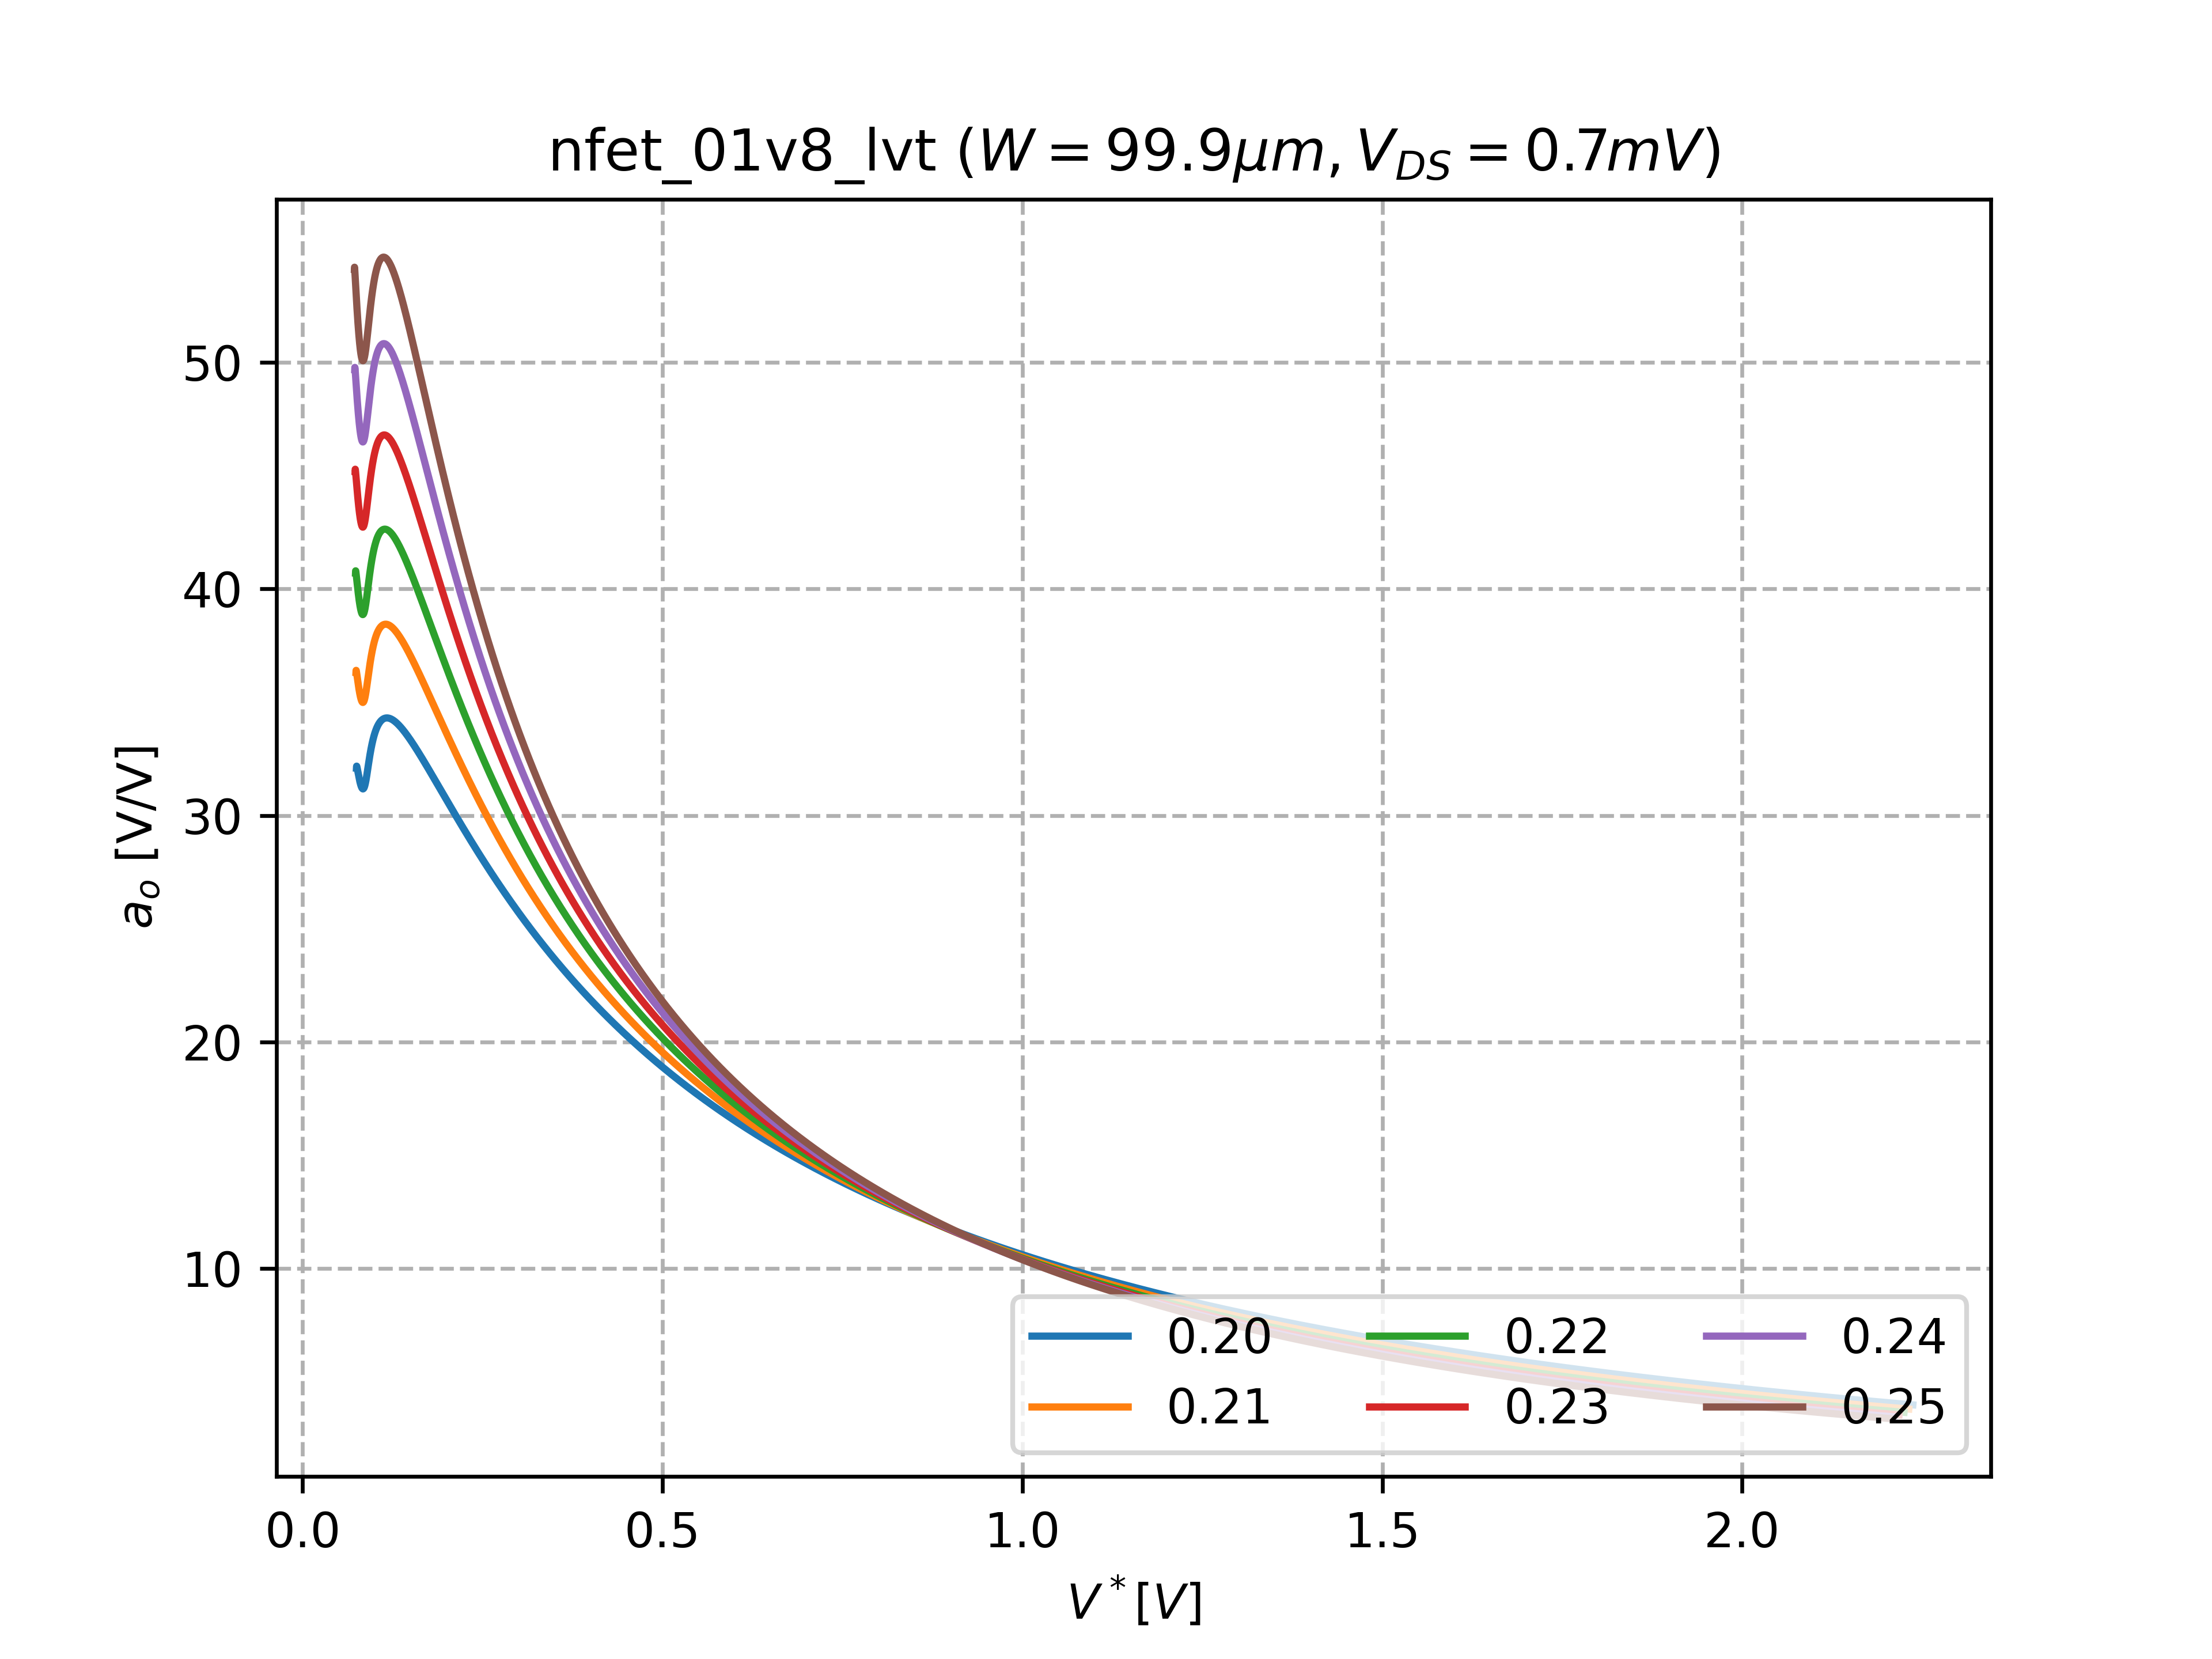
\includegraphics[width=\columnwidth]{vstar-ao-maxft.png}
	\caption{Intrinsic gain}
	\label{vstar-ao-2}	
\end{figure}
Since we need $a_o > 40$, only lengths $\geq 0.22\mu m$ can be used. 

\vspace{8pt}
\subsubsection{$f_t$ vs $V^*$} 
To trim down the possible options, we use the plot below. 
\begin{figure}[H]
	\centering 
	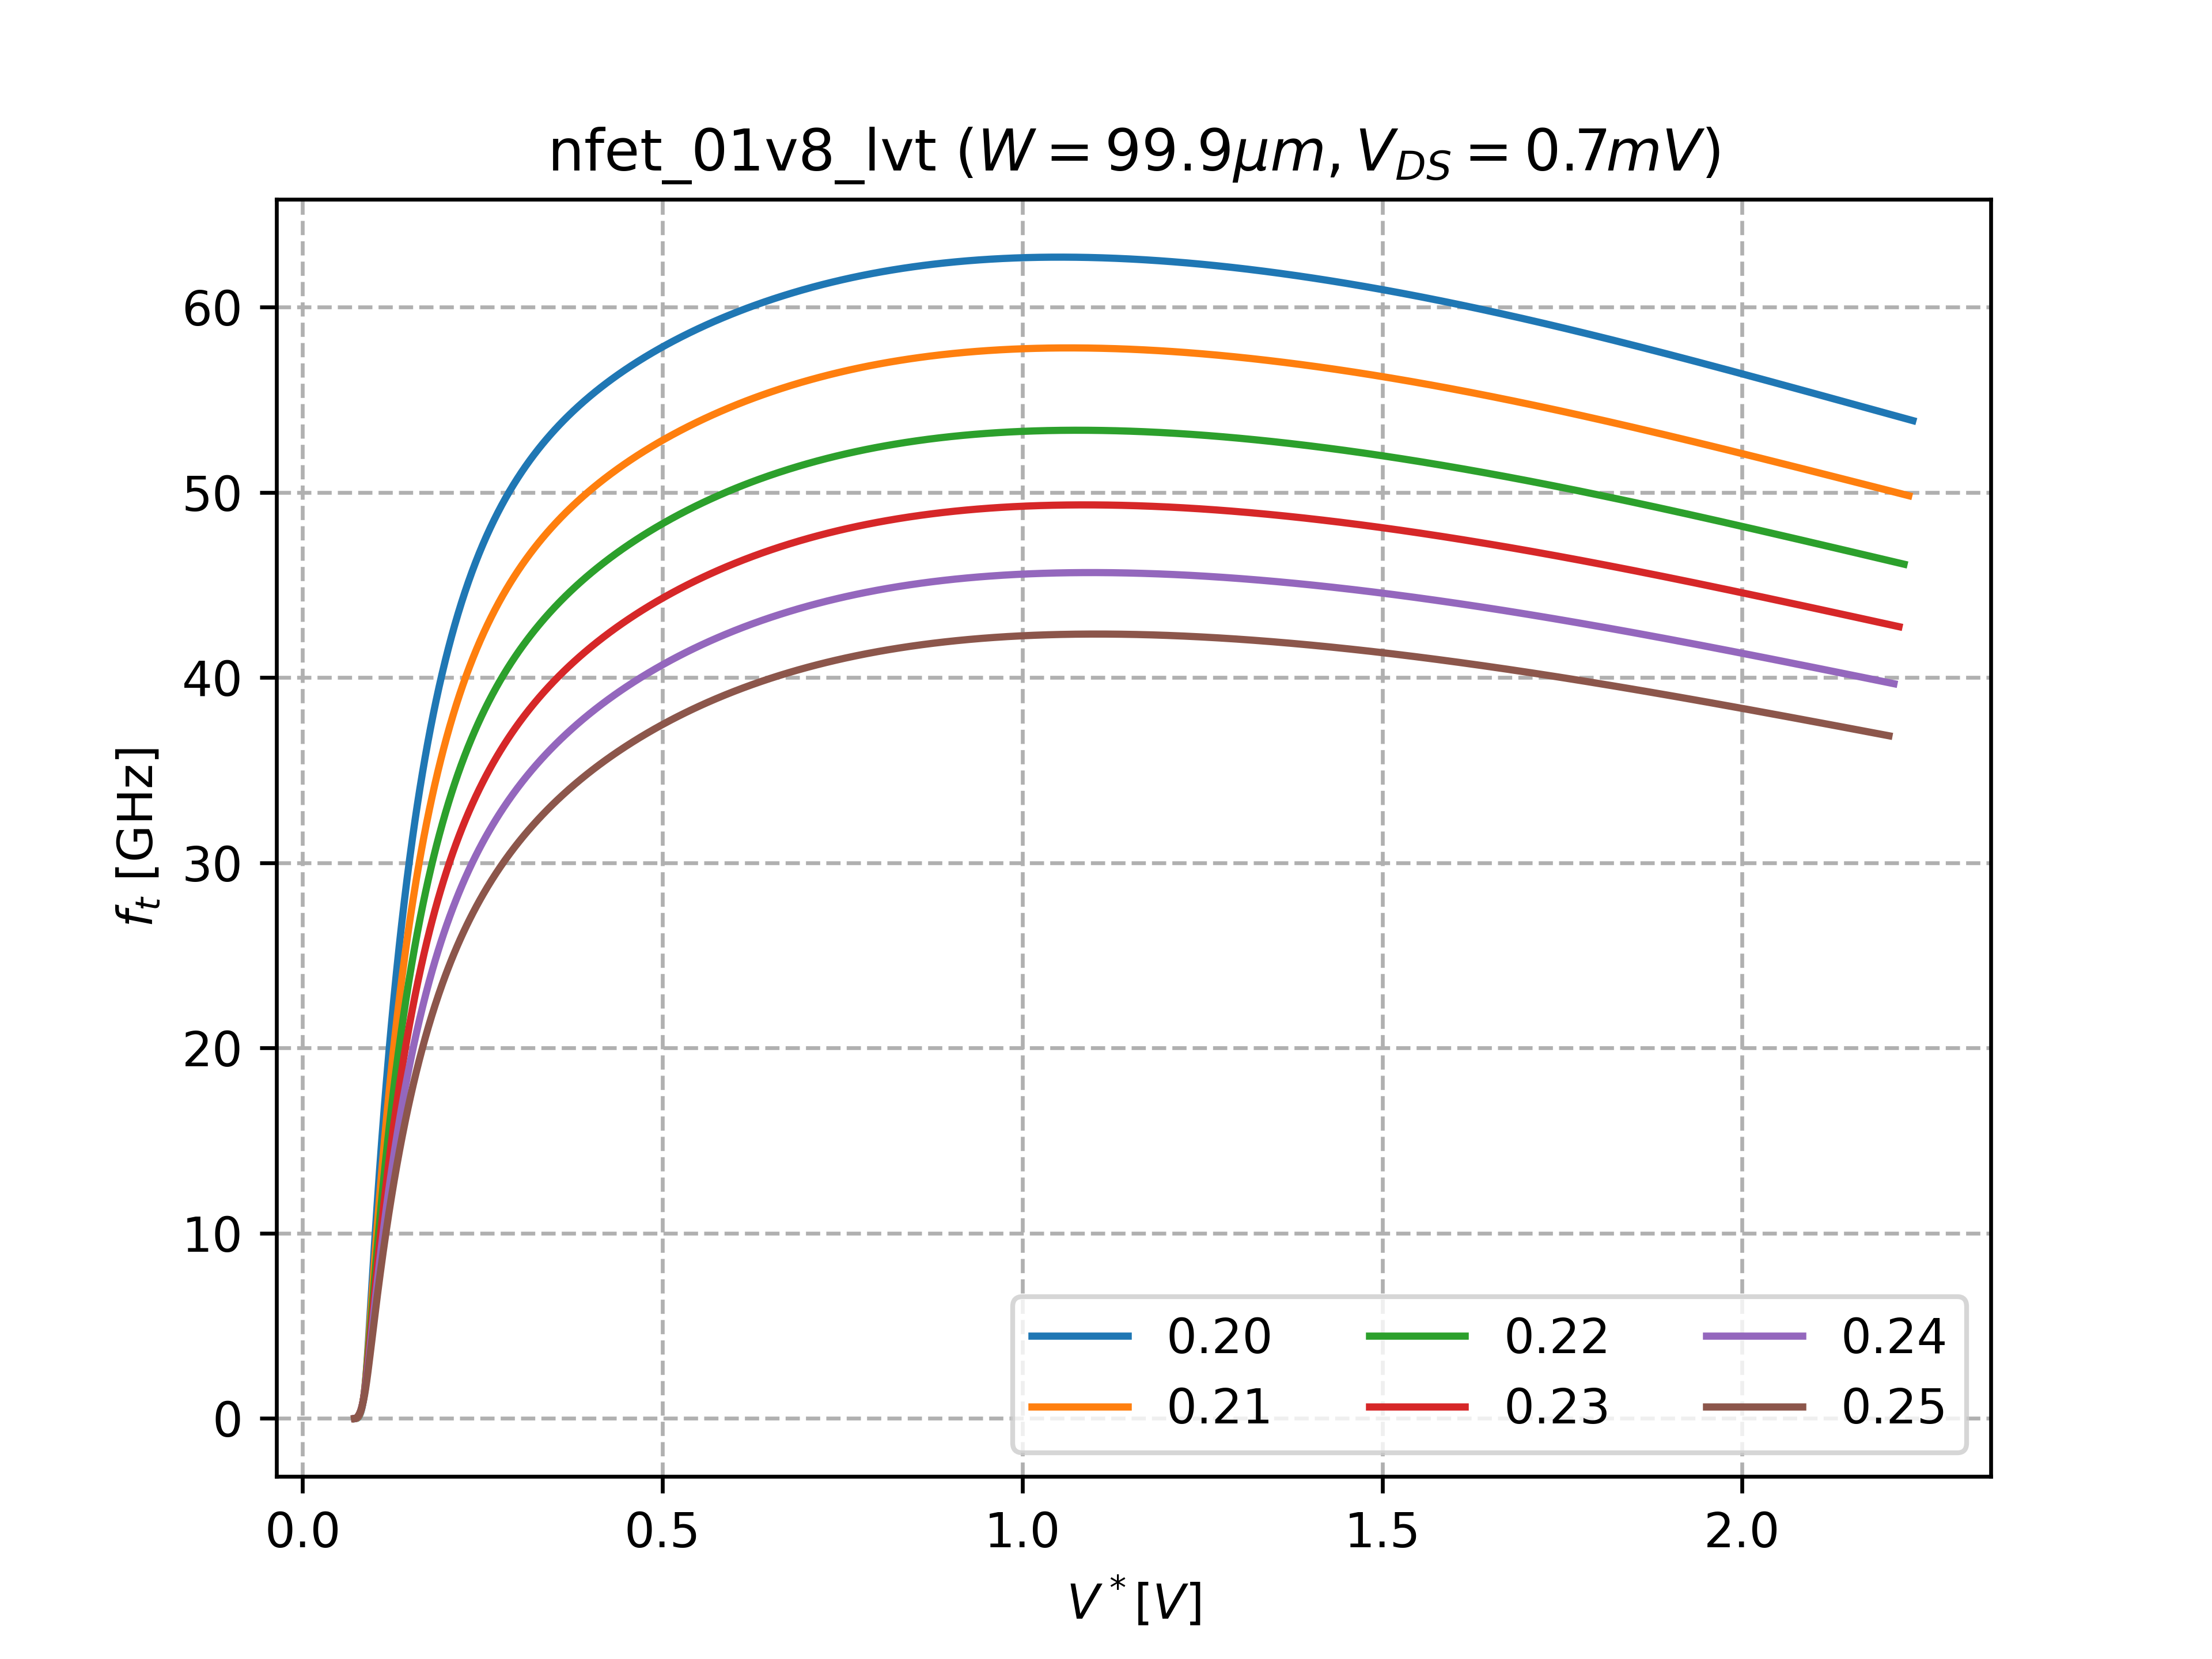
\includegraphics[width=\columnwidth]{vstar-ft-maxft.png}
	\caption{Transition frequency}
	\label{vstar-ft-2}	
\end{figure}
Considering the two plots, we choose $V^*=0.19V$ and $L=0.23\mu m$ since it has the best $f_t$. The gain and swing at these values are also within the desired specifications. 




\end{document} 
